\chapter{Image segmentation} \label{chpt:imgseg}
As introduced in Section \ref{sec:contrib}, cell tracking is an essential task for studying cell motility on a phenotypic level.

For the cell tracking methods which separate the segmentation and association steps, the segmentation quality influences the whole tracking result significantly. A highly accurate segmentation for the objects in each frame is very important, especially in the very early frames. Because the segmentation results of prior frame affects the segmentation results of later frames, miss-segmentation of an object will be hardly tracked in later frames.

Image segmentation typically is an \emph{ad-hoc} problem, in the sense that each type of data set requires choosing and adapting computational methods suitable for the characteristics of the given data. Different segmentation approaches emphasize one or more of the desired properties. During the past 40 years, hundreds of segmentation algorithms have been proposed \cite{freixenet2002yet}. Some basic segmentation methods, such as global/local thresholding and some complex segmentation models, such as active contours, Chan and Vese's method , and graph-cut method, will be introduced in this chapter.

While Sections \ref{sec:thresh_method}-\ref{sec:levelsetseg} reviews existing approaches and underlying concepts, Section \ref{sec:vdlst} introduces a novel level-set based approach for multiple object tracking.More precisely, I propose a Voronoi diagram based multi-cell segmentation method, which needs only one level set function. It is an extension of Dufour \cite{dufour2005segmenting} and Zhang's method \cite{zhang2004tracking} without considering the coupling constraints (usually unnecessary). The key idea of my method is to build a Voronoi diagram for all cells by using the fast marching method. Then each object performs the Chan Vese's segmentation method in its own Voronoi area. I build an image processing platform with lots of image segmentation algorithms in C/C++, which is distributed as an open source repository.
\section{Thresholding method} \label{sec:thresh_method}
\subsection{Overview}
In digital image processing, thresholding is the most commonly used technique for image segmentation due to its easy usage. Normally the thresholding value is a single intensity value which partitions a grayscale image into foreground and background area. It is often an effective tool to separate objects from the background and it is always the first tried method before applying other complex segmentation methods. One application of thresholding is document image analysis which aims to extract printed characters \cite{kamel1993extraction,abak1997performance}, graphs, or other items. Examples of thresholding applications lie in all kinds of pre-processing or post-processing steps, including edge detection, image feature extraction, distance transform, skeleton extraction, cell tracking to mention only a few prominent examples. In practice, thresholding can solve most problems. However, a good thresholding value is required.

Despite its simplicity, there is no strict definition for the thresholding of an image. Quite a lot of thresholding techniques \cite{sahoo1988survey, sankur2001image, sezgin2004survey}, more than 44 binary methods, are proposed according to different criterion. Sezgin and Sankur \cite{sankur2001image, sezgin2004survey} categorize thresholding methods into six groups based on different models, that is histogram shape-based methods, clustering-based methods, entropy-based methods, object attribute-based methods, spatial methods, and local methods. Histogram shape-based methods find the thresholding value on histogram data by separating the peaks and valleys, the representing method is Otsu's thresholding method. Clustering-based methods models the foreground and background as a mixture of two Gaussians and applies clustering methods to get the two parts. Entropy-based methods utilize the entropy of the foreground and the background regions, as well as the cross-entropy between the original and binarized image, etc. Object attribute-based methods finds a partition which is similar to the gray-level image in some attributes, such as fuzzy shape similarity, edge coincidence, etc. The spatial methods utilize the probability distribution in higher-order and/or correlation between pixels. Local methods calculate a suitable threshold value for each pixel according to the local image characteristics, such as the standard deviation, mean, etc.

As thresholding method is not the main segmentation method in this thesis, we only introduce some widely used algorithms. For global thresholding method, Otsu's method \cite{otsu1975threshold} is a very elegant method with solid mathematic formulas by minimizing the intra-class variance or maximizing inter-class variance. Further noteworthy, it is easy to extend Otsu's method into multi-thresholding method. For local thresholding, the thresholding is decided by average local gray values and/or standard variance. 
\subsection{Global thresholding and Otsu's method}
Global thresholding converts a grey-level image into binary image by turning all pixels below some threshold to zero and all pixels above that threshold to one. If $g(x,y)$ is a thresholded version of $f(x,y)$ at some global threshold $T$, 
\begin{equation}
g(x,y) = \left\{
  \begin{array}{ll}
  1 & \mbox{if } f(x,y) \ge T \\
  0 & \mbox{otherwise}
  \end{array}
  \right.
\end{equation}
To set a global threshold $T$, we usually analyse the histogram profile by finding a valley that separates two "mountains". One mountain for the foreground and one for the background. The histogram of an image is a probability distribution,
\begin{equation}
p(g) = n_g/n
\end{equation}
where, $n_g$ is the number of pixels with intensity $g$, $n$ is the total number of pixels. There are two ways to decide the global threshold, the iterative method and Otsu's method. 

\textbf{Iterative method :} This method compute the global threshold from the initial mean intensity value, then iterative replace the threshold value by the average mean intensity of the foreground and the background regions. See Alg. \ref{alg:global-thresh} for details of this method.

The main problem for the iterative method is speed. The step for segmenting an image into foreground and background for many times is time consuming.

\begin{algorithm}
\SetAlgoLined
\KwData{Grey-level image and the histogram}
\KwResult{The global threshold}
Estimate the initial threshold $T$ with the mean value.\\
Divide the image into foreground area $F$ and background area $B$.\\
Calculate the mean intensity $\mu_f$ and $\mu_b$ for area $F$ and $B$ respectively.\\
Refresh the threshold $T = (\mu_f + \mu_b)/2$\\
Repeat 2-4 until $\mu_f$ and $\mu_b$ do not change any more
\caption{Iterative method for global thresholding}
\label{alg:global-thresh}
\end{algorithm}
\textbf{Otsu's method : } Otsu \cite{otsu1975threshold} proposed a method based on selecting the lowest point between two classes. The selected point will minimize the intra-class variance or maximize the inter-class. The intra-class variance is defined as the weighted sum of variances of the foreground area and background area.
\begin{equation} \label{eq:intra-var}
\sigma_w^2(t) = w_b(t)\sigma_b^2(t) + w_f\sigma_f^2(t)
\end{equation}
where $w_f$ and $w_b$ are the probabilities of the two classes separated by threshold $t$, $\sigma_f^2$ and $\sigma_b^2$ are the variance of foreground and background regions.

Further, Otsu demonstrates that minimizing the intra-class variance is the same as maximizing inter-class variances
\begin{equation} \label{eq:inter-var}
\sigma_b^2(t) = \sigma_T^2 - \sigma_w^2(t) = w_f(t)w_b(t)[\mu_f(t) - \mu_b(t)]^2,
\end{equation}
where $\sigma_T^2$ is the total variance of the whole image, and $\mu_f$ and $\mu_b$ are the mean intensity of foreground and background regions. Here $w_b(t) = \sum_{i=0}^tp(i)$, $w_f(t) = 1 - w_b(t)$, $\mu_b(t) = \sum_{i=0}^tp(i)x(i)/w_b(t)$, and $\mu_f = (\mu_T - \mu_b(t)w_b(t))/w_f(t)$

By using formula \ref{eq:inter-var}, the Otsu's method can be written as a dynamic algorithm, and thus will be very fast. The equations for dynamic Otsu's method is as follows, 
\begin{equation} \label{eq:otsu-dynamic}
\begin{array}{lll}
	w_b(t) & = & w_b(t-1) + p(t) \\
	w_f(t) & = & \mu_T - \mu_b(t)w_b(t) \\
	\mu_b(t) & = & (\mu_b(t-1)w_b(t-1) + p(t)x(t))/w_b(t)\\
	\mu_f(t) & = & (\mu_T - \mu_b(t)w_b(t))/w_f(t)
\end{array}
\end{equation}
where $\mu_T$ is the average intensity of the whole image. See Alg. \ref{alg:otsu-thresh} for the details. If there are multiple maximum $\sigma_b(t)^2$, the threshold value can be set as the average of them.
\begin{algorithm}
\SetAlgoLined
\KwData{Grey-level image and the histogram}
\KwResult{The global threshold}
Compute the histogram and probabilities $p(g)$ for each intensity level $g$\\
Initialize $w_i(0)$ and $\mu_i(0)$\\
Step through all possible thresholds one by one, compute $\sigma_b(t)^2$ according to eqn.\ref{eq:inter-var} and eqn.\ref{eq:otsu-dynamic}\\
Find the threshold correspond to the maximum $\sigma_b^2(t)$
\caption{Otsu's method for global thresholding}
\label{alg:otsu-thresh}
\end{algorithm}
\subsection{Local thresholding method}
Local thresholding method adapt the threshold value on each pixel to the local image characteristics \cite{kallergi1992image}, e.g. local average intensity and local intensity variance. The major problem with global thresholding is that it considers only the intensity, not any relationships between the pixels or any local characteristic. For example global thresholding can't handle changing illumination. It can give poor results for certain types of images. And the pixels identified by the thresholding process are not at all continuous. By applying a local thresholding approach, we can overcome some of the problems.

Local thresholding divides an image into sub-images by a sliding window. For each sub-image, we find its global threshold. If the region is constant, consider it against a global threshold (all black or white). If there is sufficient variance, use Otsu/Iterative method in the window. 

Generally speaking, the local threshold is set according to the local mean and local variance.
\begin{equation}
T_{local} = a\cdot\mu_{local} + b\cdot\sigma_{local}
\end{equation}
in which the coefficient $a$ for $\mu_{local}$ and the coefficient $b$ for $\sigma_{local}$ is decided according the illumination gradient or by experience.
\subsection{Component tree based thresholding} \label{sec:thresh-cptree}
A component tree of an image maintains the inclusion relationship between all possible connected component under all different threshold segmentation. When an image displays complex structures or large number of objects, the limitation of thresholding methods become very obvious. Typically, we cannot use a single threshold to identify the objects we are interested, especially when there are multiply objects, where each object lies in different gray levels. In such case, some objects will get miss-segmented or half-segmented. Another example is when the background is not evenly distributed, such as vignetting background, which is due to uneven illumination, or linear gradient of background inhomogeneity. One single threshold will inevitably divide the background area into foreground area.

Even though the local thresholding can overcome some of the problem in global thresholding, but it is not easy to decide the size of sliding windows and the coefficients. In our contribution, we use a much more advanced method which considers all possible thresholds. We will get all possible connected components under different thresholds. It is easy to see that, the relationship between connected components is either an inclusion or non-overlapping. Thus, the connected components can be represented as a tree, called the \emph{component tree}, to manage the relationship for all connected-components. 

When using the component tree, we do not have to bother about the best threshold. We can filter out the components using size or criteria, which is obtained from a prior knowledge. Details about component tree based segmentation will be introduce in Chapter \ref{chapter:cptree}.

\section{Snake: Active contour method} \label{sec:snake}
\subsection{Overview}
The active contour model \cite{kass1988snakes} (also called snake model) is popular in computer vision, which finds the object boundaries either continuous or non-continuous. It is widely used in applications like image segmentation, object tracking, shape recognition, edge detection, and stereo matching.

A \emph{snake} in the image is a sequence of discrete points, which is called a spline.
\begin{equation}
v(s) = (x_s, y_s)
\end{equation}
where $s \in [0,1]$. The snake is guided by many forces which maybe external forces from the image gradient or the internal forces from the snake curve itself. When reaching a certain equilibrium, the snake will be guided to the image boundaries and stopped.

To describe the snake state, each state (position) of the snake has an energy, which is the sum of external energy and internal energy, corresponding to it. The internal energy $E_{int}$ of the spline (snake) is due to bending. Then the external energy $E_{ext}$ consist of the image forces $E_{img}$ acting on spline and the constrained forces $E_{con}$ introduced by user. 
\begin{equation}
E_{snake} = \int_0^1E_{snake}(v(s))ds = \int_0^1(E_{ext} + E_{int})ds \\
\end{equation}
\begin{equation}
E_{ext} = E_{img} + E_{con}.
\end{equation}
While all these energy terms depend on the position s, we omit this to keep notation shot.  
\textbf{Internal energy: } The bending forces of the snake come from the curve length and curve curvature.
\begin{equation}\label{eqn:int-energy}
E_{int} = (\alpha(s)|v_s(s)|^2 + \beta(s)|v_{ss}(s)|^2)/2
\end{equation}
where $\alpha(s)$ and $\beta(s)$ controls the energy sensitive to snake stretching and curve roundness, $|v_s(s)|^2$ represents the snake length and $|v_{ss}(s)|^2$ represents the total curvature. The larger the value of $\alpha(s)$, the more sensitive of the internal energy as the snake stretches. And the larger the value of $\beta(s)$, the more sensitive of the internal energy as the curve increase.

\textbf{Image forces: } The forces have three components that is lines, edges and terminations.
\begin{equation}
E_{img} = w_{line}E_{line} + w_{edge}E_{edge} + w_{term}E_{term}
\end{equation}
The line component is just the intensity of the image
\begin{equation}
E_{line} = I(x,y).
\end{equation}
Edges in the images will make the snake attract to the area with large image gradients
\begin{equation}
E_{edge} = -|\nabla I(x,y)|^2.
\end{equation}
Or the edge computed on the Gaussian blur-ed image,
\begin{equation}
E_{edge} = -|G_\sigma \cdot \nabla^2 I|^2
\end{equation}
The termination component of energy can be defined as
\begin{equation}
E_{term} = \frac{\partial \theta}{\partial n_\perp} = \frac{C_{yy}C_x^2 - 2C_{xy}C_xC_y + C_{xx}C_y^2}{(C_x^2 + C_y^2)^{3/2}},
\end{equation}
where $C(x,y)$ is the Gaussian smoothed image on $I(x,y)$, $C_x$ and $C_y$ are gradient along $x$ and $y$, $C_{xx}$, $C_{xy}$, and $C_{yy}$ are second order gradients. This component is used to detect corners and terminations in an image.

\textbf{Constraint energy: } In some systems, the user interaction on the snake can guide the snake towards or away from particular features. 
\subsection{Energy minimization model}
The snake will move toward the energy decreasing direction. One of the simplest optimization method is gradient-descent minimization \cite{snyman2005practical}. The energy of the snake can be estimated by using the discrete points on the snake through 
\begin{equation}
E_{snake} \approx \sum_{i=1}^nE_{snake}(\bar{v}_i).
\end{equation}
Thus, the derivative of the energy can be approximated as
\begin{equation}
\nabla E_{snake} \approx \sum_{i=1}^n \nabla E_{snake}(\bar{v}_i).
\end{equation}
Now, applying the gradient descent minimization, the position of the snake is adjust as
\begin{equation}
\bar{v}_i = \bar{v}_i - \nabla E_{snake}(\bar{v}_i).
\end{equation}
This equation is applied iteratively until the energy does not change anymore.
\subsection{Other implementations}
The classical snake modes which drive the snake towards object contours depends very much on the initial snake position.
The initial snake position should be close to the object or inter-cross with object boundary. Otherwise, the snake may
get stuck in local mini-ma states and mis-finding the object. To overcome the initial position problem, many variations
based on snake model are proposed.

\textbf{Gradient Vector Flow (GVF) active contours: } In normal snake modes, the diffuse forces exist only on the object boundary. This 
makes the snake hard to converge to the object boundary. Due to this reason, the GVF active contour proposed a way to diffuse
the edge force to its surrounding, which provides a new external field. Under such model, even if the snake is started far from the object, it still gets attracted 
towards the object\cite{xu1998snakes}.

\textbf{Balloon snake: } The ballon snake \cite{kass1988snakes} behaves like a blowing ballnoon. When it passes by strong contour, it stops. Thus, the
initial snake need not to be too close to the object. The external field is modified and a new pressure force is introduced to make the curve evolve like a ballon.

\textbf{Diffusion snakes: } The diffusion snake \cite{cremers2002diffusion} is modified from Mumford-Shah \cite{mumford2006optimal} for spline contours. It is used 
when the prior shape information is known. The obtained segmentation maximizes both the Grey value homogeneity in the separated regions and the similarity of the contour with respect to a set of training shapes.

\textbf{Geometric Active Contours: } Geometric active contour \cite{malladi1995shape} proposed an energy function by summing up the snake perimeter and an inversed edge function. Through minimizing the energy function, the snake moves towards the perimeter shrinking direction and stops at the high edge area. The model may be implemented using level sets, which will be introduced in next section. For the model, the snake can be initialized relatively large to enclose the objects.
\section{Level set based segmentation} \label{sec:levelsetseg}
The level set method is a numerical method for the evolution of curve (or interface) originally introduced by Sethian and Osher \cite{malladi1995shape}. In mathematics, a level set of a function $f$ with $n$ variables is the set of the form,
\begin{equation}
LS_c(f) = \{(x_1,\ldots,x_n)|f(x_1,\ldots,x_n) = c\}
\end{equation}
where $c$ is the level set value. The level set can be used to represent a curve implicitly. For example, the two dimension circle $x^2 + y^2 = 1$ can be considered as the zero level of function $f(x,y) = x^2 + y^2 - 1$. With level set function, we can easily define the inside area, background area and interface $\Gamma$.
\begin{equation}
\Gamma = \{\vec{x}|f(\vec{x}) = 0\}
\end{equation}
\begin{equation}
Inside = \{\vec{x}|f(\vec{x}) > 0\}
\end{equation}
\begin{equation}
Outside = \{\vec{x}|f(\vec{x}) < 0\}
\end{equation}

The great advantage of level set methods is the ability to utilize the regional information, such as the area and average intensity properties. Based on such merits, Chan and Vese \cite{chan2001active,chan2000active} proposed a modified Mumford-Shah functional to segment an image into piecewise constant regions without considering the edge information. However, the Chan-Vese model can only segment an image into two phases (two distinct regions), which makes it is hard to distinguish multiple-objects. To overcome break this limitation, a multi-phase level set method \cite{vese2002multiphase} is proposed to segment an image into $N$ phases with $\left \lfloor \log_2N \right \rfloor$ level set functions, where each phase represents an object. Furthermore, to overcome the cell touching problem, the coupled level set model was proposed by Zhang \cite{zhang2004tracking} to segment $N$ objects with $N$ level set functions. Dufour \cite{dufour2005segmenting} extends the model to 3D confocal image segmentation. Palaniappan \cite{nath2006robust} introduced an approach that reduced the number of level set functions to only four.

\subsection{Explicit methods vs. implicit methods}
Usually there are two ways to represent a curve, explicitly or implicitly. The explicit way defines a curve through vertices along the curve, i.e., 
\begin{equation}
C = \{C_i| C_i=(x_i, y_i), i \in \{1,\ldots,n\}\},
\end{equation}
where $n$ is the vertex number on the curve, $C_0$ is the start point and $C_n$ the last point. The implicit way defines a curve as the zero level set of a function,
\begin{equation}
C = \{(x,y)|f(x,y) = 0\}
\end{equation}
The solution for an explicit curve is explicit method, and the solution for an implicit curve is implicit method. 

\emph{Explicit methods} calculate the state of a curve at a later time from the state of the curve at the current time, while \emph{implicit methods} find a solution by solving an equation involving both the current state of the curve and the later one. Let $C(t)$ stands for current curve state and $C(t+\Delta t)$ is the state at the later time, then, for an explicit method
\begin{equation}
C(t+\Delta t) = F(C(t))
\end{equation}
while for an implicit method one solves an equation
\begin{equation}
G(C(t), C(t+\Delta t)) = 0
\end{equation}
to find $C(t + \Delta t)$.

Obviously, the implicit method will need more computation time and is generally hard to implement. However, with level set method the implicit methods have many great feature. Without having to parametrize these objects, the level set method enables an easy way to follow shapes that change topology, such as shape splitting, shape merging, and adding holes. As many fast algorithms appeared, the limitation of level set method becomes less important. 

For some segmentation problems, such as the Chan-Vese model described, it impossible to use explicit methods when the regional information is considered, while implicit methods solve the problem naturally.
\subsection{Chan-Vese model}
Based on the level set curve evolution and Mumford-Shah function, Chan and Vese \cite{chan2001active} proposed a new model for active contours to detect objects in an image. The model can detect objects whose boundary is free of so-called sharp edges. Though without edges, the evolving curve can still stop at the desired position by minimize an energy function. With level set technique, the Chan-Vese model overcomes many difficulties arising in previous methods (snake model) of image segmentation.

The Chan-Vese model considers the segmentation result of an image $u_0$  as a piecewise constant image $u$. The foreground (inside) area of $u$ is of constant intensity $c_i$, and the background (outside) area of $u$ is of constant intensity $c_o$. The energy function for the segmentation result $u$ is defined as the difference between $u_0$ and $u$.
\begin{eqnarray*}
E(C) & = &  \int_{inside( C)}|u_0(x,y) - c_i|^2dxdy + \int_{outside( C)}|u_0(x,y) - c_o|^2dxdy
\end{eqnarray*}
Here, $C$ is the segmentation contour (curve), which is the zero level set of a function $\phi$,
\begin{equation}
C = \{(x,y) \in \Omega|\phi(x,y) = 0\}
\end{equation}
And the inside and outside area is defined as the positive level sets and negative level sets of $\phi$.
\begin{equation}
inside( C) = \{(x,y) \in \Omega|\phi(x,y) > 0\}
\end{equation}
\begin{equation}
outside( C) = \{(x,y) \in \Omega|\phi(x,y) < 0\}
\end{equation}
For the constant values $c_i$ and $c_o$,  they can be user defined intensity or the average intensity of inside and outside area,
\begin{equation}
c_i(\phi) = \frac{\int_{\Omega}u_0(x,y)H(\phi(x,y))dxdy}{\int_{\Omega}H(\phi(x,y))dxdy}
\end{equation}
\begin{equation}
c_o(\phi) = \frac{\int_{\Omega}u_0(x,y)(1-H(\phi(x,y)))dxdy}{\int_{\Omega}(1-H(\phi(x,y)))dxdy}
\end{equation}
where $H(z)$ is a binary function, that is one for positive value and zero for negative value.

To get a so that smoother boundary, we can add more regularizing items to the energy function,
\begin{eqnarray}
\label{eqn:chanvese}
E(c_i,c_o,C) & = & \mu\cdot\mbox{Length( C)} + \nu \cdot \mbox{Area} + \lambda_1\int_{inside( C)}|u_0(x,y) - c_i|^2dxdy \\
\nonumber
& & + \lambda_2\int_{outside( C)}|u_0(x,y) - c_o|^2dxdy.
\end{eqnarray}

This energy function is an extension of geometric active contour model by minimize the perimeter of the contour. Here the length and area energies are defined as, 
\begin{equation}
\mbox{Length}\{\phi = 0\} = \int_\Omega|\nabla H(\phi(x,y))|dxdy = \int_{\Omega}\delta_0(\phi(x,y))|\nabla\phi(x,y)|dxdy
\end{equation}
\begin{equation}
\mbox{Area}\{\phi \ge 0\} = \int_{\Omega}H(\phi(x,y))dxdy
\end{equation}
where $\delta_0(z) = \frac{d}{dz}H(z)$ and $\Omega$ is the image domain.

\subsubsection{Numerical solution}
Equation \ref{eqn:chanvese} is solved by a variational method. Through substituting into the Euler-Lagrange equation and applying Green's identity and Green's theorem, the solution PDE is,
\begin{equation}
\frac{\partial \phi}{\partial t} = \delta(\phi)\left[\mu\mbox{div}\left(\frac{\nabla\phi}{|\nabla\phi|}\right)-\nu -\lambda_1(u_0-c_1)^2 + \lambda_2(u_0-c_2)^2\right]
\end{equation}

\subsubsection{Effect of weights}
Each energy term in eqn. \ref{eqn:chanvese} is weighted according to real instance. 
\begin{itemize}
\item[(a)] For length energy weight, $\mu$ controls the smoothness of the contour. High $\mu$ value enables a tightly attached contour to the object, whereas low $\mu$ value enables a loosely enclosed contour. 
\item[(b)] The area weight $\nu$ inhibit the growing of inside area. 
\item[(c)] The relative balance between $\lambda_1$ and $\lambda_2$ determines which side, inside or outside, has higher importance in minimizing the energy. 
\end{itemize}

\subsubsection{Generalizing to N-dimension}
Chan-Vese model can be naturally extended to N-dimensional image segmentation with the energy function,
\begin{eqnarray}
\nonumber
E(\phi, c_i, c_o) & = & \mu\int_\Omega |\nabla H(\phi(\vec{x}))|d\vec{x} + \nu\int_\Omega H(\phi(\vec{x}))d\vec{x}\\
                 &    & + \lambda_1\int_\Omega |u_0(\vec{x} - c_i)|^2H(\phi(\vec{x}))d\vec{x} \\
\nonumber
				 &    & + \lambda_2\int_\Omega |u_0(\vec{x} - c_o)|^2(1 - H(\phi(\vec{x})))d\vec{x}
\end{eqnarray}
And the solution is similarly,
\begin{equation}
\frac{\partial \phi(\vec{x})}{\partial t} = \delta_0(\phi(\vec{x})\left[\mu\mbox{div}\left(\frac{\nabla\phi(\vec{x})}{|\nabla\phi(\vec{x})|}\right)-\nu -\lambda_1(u_0(\vec{x})-c_i)^2 + \lambda_2(u_0(\vec{x})-c_o)^2\right] 
\end{equation}

\subsubsection{Generalizing to vector-valued images}
For an image with multiple channels (RGB image), each pixel is a vectorized value. The energy is defined as the average energy of each channel \cite{chan2000active},
\begin{eqnarray}
\nonumber
E(\phi,\vec{c^+}, \vec{c^-},\phi) & = &\mu\cdot L + \int_{inside( C)} \frac{1}{N}\sum_{i=1}^N\lambda_i^+|I_i(x,y)-c_i^+|^2dxdy \\
& & + \int_{outside(C )}\frac{1}{N}\sum_{i=1}^N\lambda_i^-|I_i(x,y)-c_i^-|^2dxdy
\end{eqnarray}
where $\vec{c^+}$ and $\vec{c^-}$ are inside average intensity and outside average intensity for each channel with the same segmentation result $\phi = 0$. The corresponding solution reads a
\begin{equation}
\frac{\partial \phi}{\partial t} = \delta(\phi)\left[\mu\mbox{div}\left(\frac{\nabla\phi}{|\nabla\phi|}\right) -\frac{1}{N}\sum_{i=1}^N\lambda_i^+(I_i(x,y)-c_i^+)^2 + \frac{1}{N}\sum_{i=1}^N\lambda_i^-(I_i(x,y)-c_i^-)^2\right].
\end{equation}

For the vector-valued Chan Vese model, besides its application to RGB images, it can be used for texture image segmentation. A texture image can be decomposed into many small blocks, where for each block many features are being calculated. Thereby a texture image can be converted into a low resolution image with many channels (that is, one feature one channel).

\subsection{Multiple object segmentation}
The Chan-Vese model segments an image into two phases, the interested cells are all segmented into one region, which is hard to distinguish. Later, a multiphase variant of the Chan-Vese model was proposed to handle $2^n$ unique phases with $n$ level set functions. However Zhang \cite{zhang2004tracking}, Dufour \cite{dufour2005segmenting} and Zimmer \cite{zimmer2005coupled} found that the multi-phase model is unsuitable for realiable cell segmentation due to the problem of frequent cell merging. By considering the merging event, Zhang \cite{zhang2004tracking} proposed an $N$-level set framework, that each level set function describes an object, by adding a coupling punishment for merging areas. The following two sections will introduce multi-phase level set methods and the coupling level sets method.

Some practical experiments have been conducted as part of this thesis. As it turns out, the coupling constraints are not very helpful. Most likely, this is because, the coupling weights are difficult to determine. To explain the difficulties of using coupling constraints in practice, I summarize the observations from these experiments in a rather anecdotal manner. The coupling area usually changes dramatically. For an unsuitable coupling weight, the coupling area disappears rapidly once two cells merged together. For a reason, we can force the level set function stop growing when meet with the boundary of another level set function. Thus, we can set a boundary for each level set function according to the initial object area. Such boundary could actually be obtained from a generalized Voronoi diagram of all input objects. After that, we can perform Chan-Vese's level set method in each Voroni area. The Voronoi diagram changes every a few iterations according the last level set segmentation results. With Voronoi diagram, we will need only one level set function to segment any number of objects. 

\subsection{Multiphase level sets method}
To segment multiple objects, Chan and Vese extended their 2-phase algorithm to an $N$-phase algorithm by using $\left \lfloor \log_2N \right \rfloor$ level set function. Because, $n$ level set functions could form $2^n$ inter-crossing region. Each object is described as the combination of inside or outside of these level set functions. For example, an image $u_0$ can be segmented into four areas with two level set function $\phi_1$ and $\phi_2$. The four areas are,
\begin{equation}
u_{00} = \{(x,y) | H(\phi_1(x,y)) == 0 \&\& H(\phi_2(x,y)) == 0\}
\end{equation}
\begin{equation}
u_{01} = \{(x,y) | H(\phi_1(x,y)) == 0 \&\& H(\phi_2(x,y)) == 1\}
\end{equation}
\begin{equation}
u_{10} = \{(x,y) | H(\phi_1(x,y)) == 1 \&\& H(\phi_2(x,y)) == 0\}
\end{equation}
\begin{equation}
u_{11} = \{(x,y) | H(\phi_1(x,y)) == 1 \&\& H(\phi_2(x,y)) == 1\} 
\end{equation}
Here, the four regions $u_{00}$, $u_{01}$, $u_{10}$, and $u_{11}$ are partitions of image $u_0$. The energy function is defined as the sum of energy (variance) in each regions and the sum of length of the boundary.
\begin{eqnarray}
\nonumber
E(\phi_1,\phi_2, \vec{c}) & = & \mu_{00}\int_{\Omega}(u_0(x,y) - c_{00})^2(1-H(\phi_1))(1-H(\phi_2))dxdy \\
\nonumber
& & + \mu_{01}\int_{\Omega}(u_0(x,y) - c_{01})^2(1-H(\phi_1))H(\phi_2)dxdy \\
\label{eqn:4phase}
& & + \mu_{10}\int_{\Omega}(u_0(x,y) - c_{10})^2H(\phi_1)(1-H(\phi_2))dxdy \\
\nonumber
& & + \mu_{11}\int_{\Omega}(u_0(x,y) - c_{11})^2H(\phi_1)H(\phi_2)dxdy \\
\nonumber
& & + \sum_{1 \le i \le 2}\nu_i\int_{\Omega}|\nabla H(\phi_i)|dxdy
\end{eqnarray}
where $\mu_{ij}$ is the weight of energy for each region, $\vec{c}$, which contains $c_{00}$, $c_{01}$, $c_{10}$ and $c_{11}$, is the mean of each region, $\nu_i$ is the weight for the length of each level set function. Through the above Euler-Lagrange equation \ref{eqn:4phase}, we get the derivative functions for both $\phi_1$ and $\phi_2$, so that
\begin{eqnarray}
\frac{\partial \phi_1}{\partial t}  & = &  \delta_0(\phi_1) [\mu_{00}|u_0 - c_{00}|^2(1-H(\phi_2)) + \mu_{01}|u_0 - c_{01}|^2H(\phi_2) \\
\nonumber
 & & - \mu_{10}|u_0 - c_{10}|^2(1-H(\phi_2)) - \mu_{11}|u_0 - c_{00}|^2H(\phi_2) +\nu_1\nabla(\frac{\nabla\phi_1}{|\nabla\phi_1|})]
\end{eqnarray}
\begin{eqnarray}
\frac{\partial \phi_2}{\partial t}  & = &  \delta_0(\phi_2) [\mu_{00}|u_0 - c_{00}|^2(1-H(\phi_1)) - \mu_{01}|u_0 - c_{01}|^2H(\phi_1) \\
\nonumber
 & & + \mu_{10}|u_0 - c_{10}|^2(1-H(\phi_1)) - \mu_{11}|u_0 - c_{00}|^2H(\phi_1) +\nu_1\nabla(\frac{\nabla\phi_2}{|\nabla\phi_2|})].
\end{eqnarray}

When extended to $N$-phases with $\left \lfloor \log_2N \right \rfloor$ level set functions, the energy function becomes
\begin{equation}
E(\Phi, \vec{c}) = \sum_{1\le i \le N} \mu_i\int_{\Omega}(u_0(x,y) - c_i)^2\chi_idxdy + \sum_{1 \le i \le \left \lfloor \log_2N \right \rfloor}\nu_i\int_{\Omega}|\nabla H(\phi_i)|dxdy,
\end{equation}
where $\Phi$ is a vector of level set functions ($\phi_1$ and $\phi_2$), $c$ is a vector of mean intensity values (i.e. $c_i = mean(u_0)$ in the region $i$), $\chi_i$ is a function used to decide whether the location $(x,y)$ is in region $i$ formed by associated Heaviside functions $H(\phi_i)$, and $\mu_i, \nu_i$ are constant weight values associated with the energy and the length terms of each level set function, respectively. 

The multi-phase level set function improves the performance of the Chan-Vese model by adding just a few ($\left \lfloor \log_2N \right \rfloor$) level set functions. In this framework, the objects with varying intensities can be segmented efficiently. But does not help to prevent under-segmentation (i.e. incorrect merges), when the objects have similar intensities (i.e. cells).

\subsection{Coupling $N$ level sets method}
To overcome the problems in multi-phase level set method, Zhang \cite{zhang2004tracking} proposed a model for segmenting $N$ cells, such that each cell is described by a level set function. The cell merging event, which happens when the inside areas of two level functions overlap, is prevented by introducing a pair-wise energy based coupling constraint. The energy function is given by
\begin{eqnarray}
\nonumber
E(\Phi, \vec{c_{in}}, c_{out}) & = & \gamma \sum_{i=1}^N\sum_{j=i+1}^N\int_\Omega H(\phi_i)H(\phi_j)dxdy + \nu \sum_{i=1}^N\int_\Omega |\nabla H(\phi_i)|dxdy\\
& & + \mu_i\sum_{i=1}^N\int_\Omega (u_0 - c_{in}^i)^2H(\phi_i)dxdy \\
\nonumber
& & + \mu_{out}\int_\Omega(u_0 - c_{out})^2 \prod_{i=1}^N(1-H(\phi_i))dxdy,
\end{eqnarray}
where $\Phi = \{\phi_1,\ldots,\phi_N\}$ represents N-level set functions, $\vec{c_{in}} = \{c_{in}^1, \ldots; c_{in}^N\}$ is the average intensities of inside area of the $N$ level set functions, whereas $c_{out}$ is the average intensity of background, which is defined as the common outside area of the $N$ level set functions. The main difference between $N$-level set model and previous (2-phase or multi-phase) Chan-Vese models is the first coupling term, where $H(\phi_i)H(\phi_j)$ characterized the overlapping between the inside areas of $\phi_i$ and $\phi_j$. This coupling term should be as small as possible. The same idea is used for 3D cell segmentation by Dufour \cite{dufour2005segmenting}. Through solving the Euler-Lagrange equation, the corresponding derivative equation for each level set function is given by
\begin{eqnarray}
\frac{\partial \phi_i}{\partial t} & = & \delta_0(\phi_i)[-\gamma\sum_{j=1, j\ne i}^NH(\phi_j) + \nu\nabla(\frac{\nabla\phi_i}{|\nabla\phi_i|}) \\
& & - \mu_i(u_0 - c_{in}^i)^2 + \mu_{out}(u_0 - c_{out})^2\prod_{j=1, j\ne i}^N(1-H(\phi_j)].
\end{eqnarray}

The novelty of this model helps to sovle the cell merging problem. However, due to the great computation cost, this method is only tested on synthetic data and some very simple data. This method is hard to be applied to large data and the effect of segmenting merging cells is not at all satisfying according to my test.

\section{V-D based level set method} \label{sec:vdlst}
The coupling based N-level set is proposed to solve the cell merging problem. However, in practice, we found that the coupling $N$ level set method can solve the cell merging problem only when there is a good initial mask. And each level set would also find other objects with similar intensity level. The biggest problem for $N$ level set model is the great computation cost, which makes the method suitable to only for small image data.

During the practice, I find that it is hard to control the overlapping area of two level set functions when the two level sets have similar intensity level. By using the coupling principal, the overlapping area appear and dispear in turns, and the overlapping area may fall apart into pieces. If the inside areas of each level set function do not overlap with each other, we can find a Voronoi area for each inside area. By doing so, each object is constrained in a small Voronoi area, without violating the area of others. We can apply Chan-Vese's method in each local area, without considering the coupling constraints. Consequently, the Voronoi boundaries need to be refreshed after a few iterations.

The energy function is defined as the sum of Chan-Vese level set energy for each Voronoi area, which is given by,
\begin{eqnarray}
\nonumber
E(\Phi,\vec{c_I},\vec{c_O}) & = & \sum_{i=1}^n \Big{\{}\mu \int_{\Omega_i} |\nabla H(\phi_i|d\vec{x} \\
\nonumber
                                                                    & + & \nu\int_{\Omega_i} H(\phi_i)d\vec{x}\\
                                                                    & + & \lambda_1 \int _{\Omega_i}|u_0(\vec{x}) - c_{I_i}|^2H(\phi_i)d\vec{x} \\
\nonumber
                                                                    & + & \lambda_2\int_{\Omega_i}|u_0(\vec{x}) - c_{O_i}|^2(1-H(\phi_i))d\vec{x} \Big{\}}
\end{eqnarray}
where $\phi_i(x) = \phi(x) * (M(x) == i)$ with the defined area $\Omega_i = \{\vec{x} \in \Omega | M(\vec{x}) == i\}$. The solution for each local level set function $\phi_i$ is,
\begin{equation}
\frac{\partial \phi_i}{\partial t} = \delta(\phi_i)\left[\mu\mbox{div}\left(\frac{\nabla\phi_i}{|\nabla\phi_i|}\right)-\nu -\lambda_1(u_0-c_{I_i})^2 + \lambda_2(u_0-c_{O_i})^2\right]
\end{equation}
The process of building the Voronoi diagram for each object is introduced in Section \ref{subsec:gvd}.

There are many advantages for V-D base one level set method. First, there is only one level set function ($\phi_i$ is just a small part of $\phi$), which saves lots of computation time. Second, it performs local segmentation, which works for images with gradient background. Third, objects with similar intensity could also be segmented.

The limitation of this model is the great dependency of the initial segmentation. However, this is also the problem of other level set methods for multi-objects segmentation. Sometimes we can use a component tree based method to get the initial segmentation by setting a suitable $mb$ value (see Section \ref{sec:cptree-applic}).

\begin{figure}[htbp]
\centering
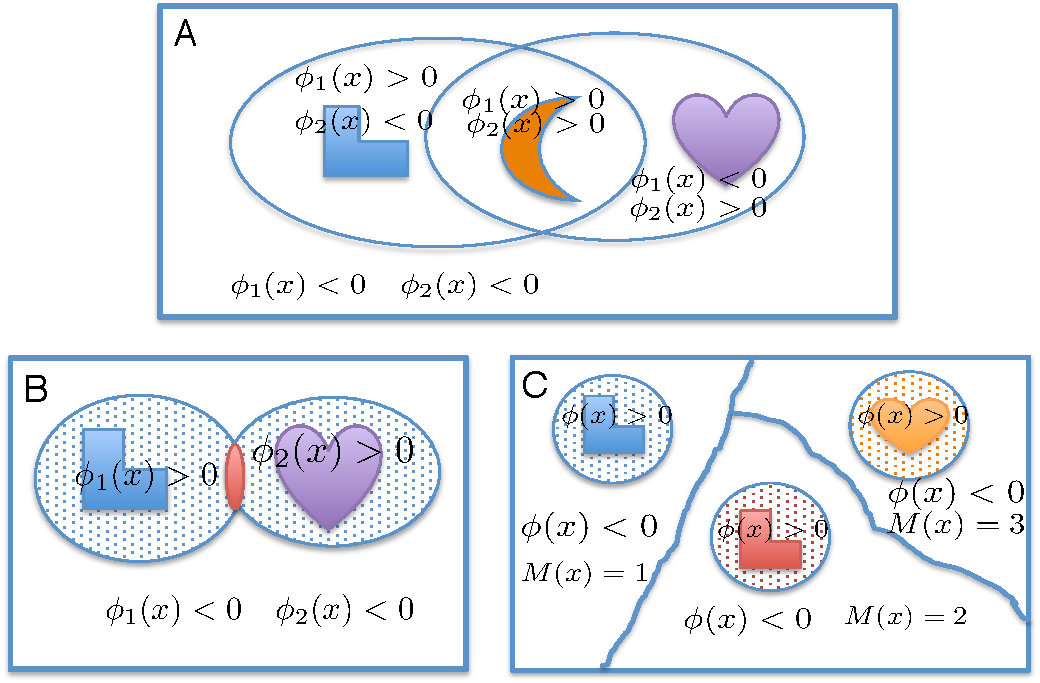
\includegraphics[width=1.0\textwidth]{images/imgseg_multiobjs}
\caption[The level set model of multi-objects segmentation]{A. Multi-phase level set model; B. Coupling $N$ level set model; C. Voronoi-Diagram base one level set model.}
\label{fig:imgseg-multiobjs}
\end{figure}
\section{Contribution of this thesis} \label{seg:imgseg-mywork}
The above image segmentation methods are from simple to complex, especially the last V-D based level set method, which is proposed by myself. I implement the method in C/C++. The test result shows its great potential on saving the running time and decreasing memory occupation significantly. In an example of segmenting an image of size 532x175 with 24 worm cells, the Dufour's method takes 11m43s, but our method takes only 24.4s which increases the speed about 29 times. The big problem which obstacles the level set method from practical use is the speed. However, our method provides a good solution.
